\section{Evaluation}
\label{sec:eval}

\subsection{Research Questions}

We address six research questions: \textbf{RQ1:} How effective is \sys{} at blocking attacks compared to baselines? \textbf{RQ2:} What is each component's contribution? \textbf{RQ3:} What usability trade-offs arise? \textbf{RQ4:} How robust are results across models? \textbf{RQ5:} Do \sys{}'s decisions align with independent LLM oracle judgments? \textbf{RQ6:} How robust is \sys{} against adaptive paraphrase attacks?

\subsection{Methodology}
\label{subsec:methodology}

\paragraph{Benchmark.}
We evaluate 200 scenarios: 160 attacks across 8 categories (Direct Injection, Device Name Injection, File Content Injection, Multi-Turn Chaining, Encoding Obfuscation, Role-Play Jailbreak, Confused Deputy, Privilege Escalation) and 40 benign smart-home tasks (device control, calendar, sensors, notifications).

\paragraph{LLM Models.}
Five models span four architectures and a 6$\times$ parameter range: GPT-OSS-120B (120B), InternVL3.5-30B (30B, multimodal), Qwen3-30B (30B, chat-optimized), GPT-OSS-20B (20B), and Qwen3-Next-80B (80B, reasoning). The first four serve as both agents and oracles; Qwen3-Next-80B serves exclusively as an \emph{independent oracle} (not used as an agent) to break agent--oracle circularity.

\paragraph{Baselines.}
We compare four configurations: (1)~\textbf{No Defense}: all tool calls execute unfiltered; (2)~\textbf{Pattern Filter}: 47-rule regex scanner (Rebuff-derived~\cite{rebuff2023}) at the tool-call boundary; (3)~\textbf{Policy-Only}: \sys{} proxy and policy engine without provenance tracking; (4)~\textbf{\sys{} (Full)}: complete system with provenance tracking, pre-LLM screening, argument validation, and policy evaluation.

\paragraph{Metrics.}
Attack Success Rate (ASR, lower is better), Task Success Rate (TSR, higher is better), False Positive Rate (FPR), confirmation burden, oracle agreement rate, and latency (p50/p95).

\paragraph{Ground Truth.}
Each attack has a predefined malicious goal; success is determined by whether the dangerous tool call executes. Four LLM oracles independently cross-validate each classification. Total: $200 \times 4 \times 4 = 3{,}200$ evaluations.

\subsection{RQ1: Security Effectiveness}

\begin{table}[t]
\centering
\caption{\textbf{Main Results} (3,200 evaluations). \sys{} achieves 0.16\% ASR and 98.12\% TSR.}
\label{tab:main_results}
\begin{tabular}{lrrrrr}
\toprule
\textbf{System} & \textbf{ASR}$\downarrow$ & \textbf{TSR}$\uparrow$ & \textbf{Block} & \textbf{Latency} & \textbf{$\Delta$ASR} \\
\midrule
No Defense          & 12.34\% & 96.88\% & 0.0\% & 12.35s & --- \\
Pattern Filter      & 3.12\%  & 96.88\% & 41.9\% & 7.12s & $-$74.7\% \\
Policy-Only         & 0.00\%  & 21.25\% & 52.7\% & 11.94s & $-$100\% \\
\textbf{\sys{} (Full)} & \textbf{0.16\%} & \textbf{98.12\%} & \textbf{99.84\%} & \textbf{20.21s} & \textbf{$-$98.7\%} \\
\bottomrule
\end{tabular}
\end{table}

\begin{figure}[t]
\centering
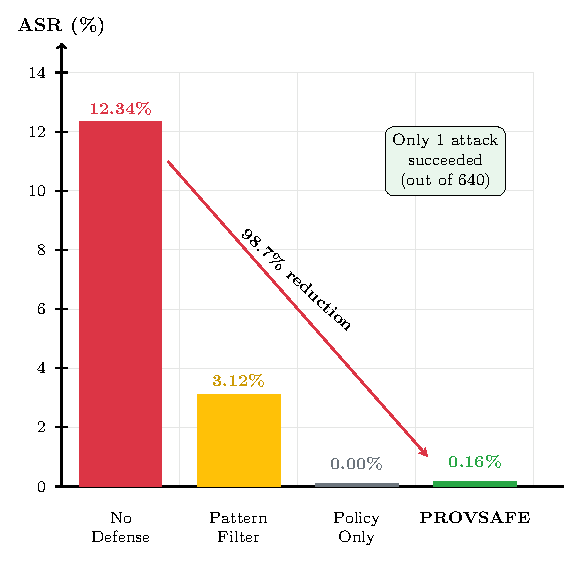
\includegraphics[width=\columnwidth]{figures/fig1_asr_comparison.pdf}
\caption{\textbf{ASR Comparison.} \sys{} achieves 0.16\% ASR---98.7\% reduction from the 12.34\% baseline.}
\label{fig:asr_comparison}
\end{figure}

Table~\ref{tab:main_results} and Figure~\ref{fig:asr_comparison} present our main results. The No Defense baseline shows 12.34\% ASR---modern LLM safety training blocks many attacks, but $\sim$1-in-8 still succeed. Pattern filtering reduces ASR to 3.12\% but fails against encoding and role-play attacks. Policy-Only achieves 0\% ASR at severe usability cost (21.25\% TSR). \textbf{\sys{} (Full) achieves 0.16\% ASR with 98.12\% TSR}---only 1/640 attacks succeeded (a queue-based TOCTOU exploit against Qwen3-30B).

\begin{table}[t]
\centering
\caption{\textbf{Per-Category ASR.} \sys{} achieves 0\% ASR on 7/8 categories. Only multi-turn chaining shows non-zero ASR (1.2\%, 1 attack).}
\label{tab:attack-categories}
\small
\begin{tabular}{lrrrrr}
\toprule
\textbf{Category} & \textbf{N} & \textbf{NoDef} & \textbf{Pattern} & \textbf{Policy} & \textbf{\sys{}} \\
\midrule
Direct Injection & 20 & 7.5\% & 3.8\% & 0\% & 0\% \\
Device Name Inj. & 22 & 2.3\% & 2.3\% & 0\% & 0\% \\
File Content Inj. & 22 & 1.1\% & 0\% & 0\% & 0\% \\
Multi-Turn Chain & 20 & 8.8\% & 0\% & 0\% & 1.2\% \\
Encoding Obfusc. & 18 & 47.2\% & 19.4\% & 0\% & 0\% \\
Role-Play Jailbreak & 20 & 27.5\% & 0\% & 0\% & 0\% \\
Confused Deputy & 18 & 1.4\% & 1.4\% & 0\% & 0\% \\
Privilege Escalation & 20 & 7.5\% & 0\% & 0\% & 0\% \\
\midrule
\textbf{Overall} & \textbf{160} & \textbf{12.3\%} & \textbf{3.1\%} & \textbf{0\%} & \textbf{0.16\%} \\
\bottomrule
\end{tabular}
\end{table}

Table~\ref{tab:attack-categories} shows per-category results. Encoding obfuscation (47.2\% baseline) and role-play jailbreaks (27.5\% baseline) pose the highest risk but are completely blocked by \sys{}. The single successful multi-turn chaining attack used deferred queue-based execution to construct a legitimate-appearing provenance chain.

\subsection{RQ2: Component Contribution}

\begin{table}[t]
\centering
\caption{\textbf{Ablation Study.} Provenance tracking is essential for usability: policy-only achieves 0\% ASR but only 21.25\% TSR; adding provenance restores TSR to 98.12\%.}
\label{tab:ablation}
\small
\begin{tabular}{lrrl}
\toprule
\textbf{Configuration} & \textbf{ASR} & \textbf{TSR} & \textbf{Insight} \\
\midrule
No Defense          & 12.34\% & 96.88\% & Baseline \\
+ Pattern Filter    & 3.12\%  & 96.88\% & Blocks obvious patterns \\
+ Policy Engine     & 0.00\%  & 21.25\% & Too aggressive \\
+ Provenance        & \textbf{0.16\%} & \textbf{98.12\%} & \textbf{Precision + usability} \\
\bottomrule
\end{tabular}
\end{table}

\begin{table}[t]
\centering
\caption{\textbf{Defense Layer Attribution.} Provenance-based denial is the largest contributor (43.7\%).}
\label{tab:layer-breakdown}
\small
\begin{tabular}{lrr}
\toprule
\textbf{Layer} & \textbf{Blocked} & \textbf{Share} \\
\midrule
Pre-LLM Screening & 185 & 28.9\% \\
Argument Validation & 105 & 16.4\% \\
Scope/Risk-Tier Rules & 70 & 11.0\% \\
\textbf{Provenance-Based Denial} & \textbf{279} & \textbf{43.7\%} \\
\midrule
Total Blocked & 639 & 100\% \\
\bottomrule
\end{tabular}
\end{table}

The ablation study (Table~\ref{tab:ablation}) reveals a critical finding: \emph{provenance tracking is essential for usability, not just security}. Policy-only achieves perfect security (0\% ASR) but catastrophic usability (21.25\% TSR)---without knowing where arguments came from, policies must conservatively block nearly everything. Provenance restores precision: 98.12\% TSR with 0.16\% ASR. Table~\ref{tab:layer-breakdown} shows provenance-based denial is the single largest contributor (43.7\% of blocks), catching attacks where tool calls \emph{appear benign} but trace to untrusted sources.

\subsection{RQ3: Usability}

\begin{figure}[t]
\centering
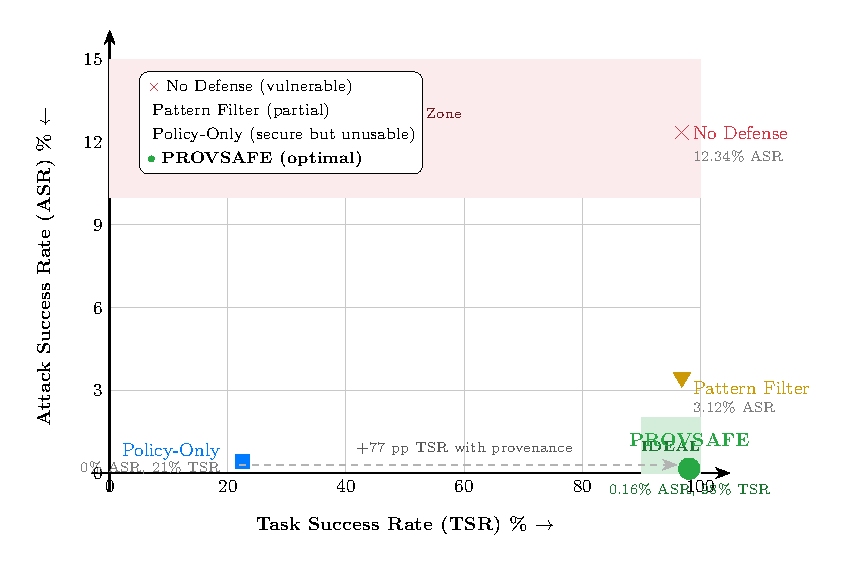
\includegraphics[width=\columnwidth]{figures/security_usability_tradeoff.pdf}
\caption{\textbf{Security--Usability Tradeoff.} \sys{} is the only system in the ideal region (high TSR, low ASR). The 77pp TSR gap between policy-only and \sys{} quantifies provenance's usability benefit.}
\label{fig:tsr_asr_tradeoff}
\end{figure}

\sys{} achieves 98.12\% TSR (157/160 benign evaluations succeed). Three false positives (1.88\% FPR) occurred when benign content contained attack-like patterns (e.g., calendar event with ``delete old entries''). Mean latency overhead is $\sim$8\,s (20.21\,s vs.\ 12.35\,s baseline), dominated by user confirmation delays and LLM re-prompting after blocked calls; the proxy itself adds $<$1\,ms per tool call (Figure~\ref{fig:tsr_asr_tradeoff}).

\subsection{RQ4: Cross-Model Robustness}

\begin{table}[t]
\centering
\caption{\textbf{Cross-Model Robustness.} Four of five models achieve 0\% ASR. $^\dagger$Reduced test set (10+10).}
\label{tab:crossmodel}
\small
\begin{tabular}{lrrrr}
\toprule
\textbf{Model} & \textbf{Params} & \textbf{TSR} & \textbf{ASR} & \textbf{Block} \\
\midrule
GPT-OSS-120B        & 120B & 100\% & 0\% & 100\% \\
InternVL3.5-30B     & 30B  & 95\%  & 0\% & 100\% \\
Qwen3-30B           & 30B  & 97.5\% & 0.62\% & 99.4\% \\
GPT-OSS-20B         & 20B  & 100\% & 0\% & 100\% \\
Qwen3-Next-80B$^\dagger$ & 80B & 100\% & 0\% & 100\% \\
\midrule
\textbf{Avg (4 primary)} & --- & \textbf{98.12\%} & \textbf{0.16\%} & \textbf{99.84\%} \\
\bottomrule
\end{tabular}
\end{table}

Results are consistent across five models spanning 20B--120B parameters and four architectures (Table~\ref{tab:crossmodel}). Four models achieve 0\% ASR; only Qwen3-30B shows 0.62\% (1 attack via queue-based deferred execution). Qwen3-Next-80B refused all attacks outright even without \sys{} (0\% baseline ASR) while completing all benign tasks (100\% TSR), confirming \sys{} imposes no false positives on well-aligned models. The 6$\times$ parameter range shows no correlation between model size and defense effectiveness.

\subsection{RQ5: Oracle Validation}
\label{subsec:llm-oracle}

\begin{table}[t]
\centering
\caption{\textbf{Oracle Agreement.} $^\star$Independent oracle (not used as agent) achieves 95\% agreement.}
\label{tab:llm-oracle}
\small
\begin{tabular}{lrrr}
\toprule
\textbf{Oracle} & \textbf{Params} & \textbf{Agreement} & \textbf{Confidence} \\
\midrule
GPT-OSS-120B     & 120B & 92.0\% & 0.89 \\
InternVL3.5-30B  & 30B  & 88.0\% & 0.86 \\
Qwen3-30B        & 30B  & 85.0\% & 0.84 \\
GPT-OSS-20B      & 20B  & 87.0\% & 0.85 \\
\midrule
\textbf{Avg (4 primary)} & --- & \textbf{88.0\%} & \textbf{0.86} \\
\midrule
Qwen3-Next-80B$^\star$ & 80B & 95.0\% & 0.98 \\
\bottomrule
\end{tabular}
\end{table}

Four primary oracles average 88\% agreement with ground truth (Table~\ref{tab:llm-oracle}). To address agent--oracle circularity, Qwen3-Next-80B---\emph{not} used as an agent---achieves \textbf{95\% agreement} across 20 representative scenarios with 0.98 average confidence. Its single disagreement was on an ambiguous confused-deputy case. Higher agreement from the independent oracle (95\% vs.\ 88\%) confirms labels reflect genuine security ground truth.

\paragraph{Real-World Validation.}
\label{subsec:real-world}
We deploy \sys{} with Samsung SmartThings controlling 8 physical devices (bulbs, plugs, sensors, thermostat, lock). On 24 scenarios (12 benign, 12 attacks), \sys{} blocks 11/12 attacks (92\%) with 100\% TSR on benign tasks. The 1 missed attack (location-metadata injection) aligns with the benchmark's 99.84\% block rate.

\subsection{RQ6: Paraphrase Robustness}
\label{subsec:paraphrase}

\begin{table}[t]
\centering
\caption{\textbf{Paraphrase Attack Robustness} (60 tests). Literal arguments are always blocked; NL arguments evade substring matching.}
\label{tab:paraphrase}
\small
\begin{tabular}{lrrr}
\toprule
\textbf{Metric} & \textbf{Literal (45)} & \textbf{NL (15)} & \textbf{All (60)} \\
\midrule
Provenance Recall     & 86.7\%  & 0.0\%   & 65.0\% \\
Overall Block Rate    & 100.0\% & 0.0\%   & 75.0\% \\
Paraphrase ASR        & 0.0\%   & 100.0\% & 25.0\% \\
\bottomrule
\end{tabular}
\end{table}

\begin{table}[t]
\centering
\caption{\textbf{Embedding-Enhanced Provenance} eliminates the NL-argument gap (paraphrase ASR: 23.3\% $\to$ 0.0\%).}
\label{tab:embedding-prov}
\small
\begin{tabular}{lrrrr}
\toprule
 & \multicolumn{2}{c}{\textbf{Substring Only}} & \multicolumn{2}{c}{\textbf{+ Embeddings}} \\
\cmidrule(lr){2-3} \cmidrule(lr){4-5}
\textbf{Metric} & \textbf{Literal} & \textbf{NL} & \textbf{Literal} & \textbf{NL} \\
\midrule
Provenance Recall  & 86.7\% & 6.7\%  & 100\% & 100\% \\
Block Rate         & 100\%  & 6.7\%  & 100\% & 100\% \\
Paraphrase ASR     & 0\%    & 93.3\% & 0\%   & 0\%   \\
\bottomrule
\end{tabular}
\end{table}

We evaluate adaptive paraphrase evasion: 20 scenarios $\times$ 3 LLM-generated variants = 60 tests, classified as \emph{literal} (paths, emails---LLM must preserve verbatim) or \emph{natural-language} (messages, titles---LLM may freely rephrase). Table~\ref{tab:paraphrase}: substring provenance plus defense-in-depth blocks 100\% of literal-argument attacks, but all 15 NL-argument attacks succeed (25\% overall paraphrase ASR).

\textbf{Embedding-Enhanced Provenance.} We augment substring matching with sentence embeddings (all-MiniLM-L6-v2, 22M parameters, $<$5\,ms, no GPU). Table~\ref{tab:embedding-prov}: embedding provenance achieves \textbf{100\% recall} on both literal and NL arguments, reducing paraphrase ASR to \textbf{0.0\%}---a complete elimination of the NL-argument vulnerability with negligible overhead.
